%
%	Begrifflichkeiten
%

\pagebreak
\section{Data Source and Wrangling}

\onehalfspacing

\subsection{Data Source}

\subsubsection{The Group}

Kölle for Future is a regional umbrella organization for a number of for-Future groups on Cologne, mainly Fridays for Future, Students for Future, Parents for Future, Grannies for Future, Teachers for Future, Psychologists for Future and Scientists for Future.

The group does not have a formal structure but follows the organizational structure of its main actors. As in most grass-roots organizations, most major decisions are made in plenary sessions; sometimes with majority voting, sometimes through consensus. The decision process is generally speaking not fast - although I got permission to perform the analysis on our blog from the Parents' plenary session, implementation of the results of this analysis will take time. Experiments, such as making changes to a form and observing the results, will need to follow the group's decision making process.

\subsubsection{The Blog}

As part of our overall social media presence and digital activism strategy, we operate a blog for KFF at the following URL: \url{https://koelle4future.de/}.

Together with our Facebook page and a number of messenger channels, the blog is the primary medium to broadcast regional news and events to all for-Futures in and around Cologne.

It is an important part of our effort to keep the groups together and engaged during the pandemic, when we cannot meet in person. Part of the KFF activism has become digital, with bi-weekly virtual rallies (aka \#DigitalStrike) that we hold on Zoom and advertise through the blog. 

In this paper, I will look at the blog's traffic data and analyze that data. The goal is to understand the performance and reach of a blog post based on its content. With this information we want to improve our outreach and better serve our community.

\subsubsection{Social Media and Loneliness}

Social distancing ("six feet apart") is the key element in containing the spread of Sars-CoV-2. Unfortunately it's also the best method to stop the spread, which is easy for some but very difficult for others.

According to a recent study conducted by the American Psychological Association, social distancing over an extended period of time can increase loneliness and significantly affect people's health.\footnote{See \textit{Luchetti, M. (2020)}: The trajectory of loneliness in response to COVID-19. \cite{apaLoneliness}}

In their study, the researchers put forward the hypothesis that an increase in support from others, perceived of real, can significantly offset that feeling of loneliness.

One means to support the members of our community is through an increase in interaction on social media. To maximize outreach, we use all kinds of channels in parallel and include a blog. We hope that the more engaging a blog post is, the better are its chances to reach people and be entertaining or otherwise beneficial. The main goals is to keep our community engaged and to combat loneliness.

Another means to reach out to our community is through virtual meetings with video. However, here we will not look into this or in any other channel than our blog.

\subsubsection{Hate Speech}

Besides loneliness, another aspect of moving to the digital realm in the Covid-19 pandemic is an increase of Hate Speech, especially in social media. It is our aim with the blog and our other platforms to offer a safe and welcoming digital space and restrict the use of hateful words in comments and the use of derogatory terms.

With Covid-10, as with any other illness, comes stigma and we need to be especially aware to not stigmatize people who have contracted the virus and might be on a long path to recovery.\footnote{See \textit{UNAIDS (2020)}: Addressing stigma and discrimination. \cite{addressingStigma}} During the pandemic, it's very important to be inclusive to all people, inside and outside of our community.\footnote{See \textit{TIME's UP (2020)}: Equity and Inclusion During Crisis. \cite{equityInclusion}}

\subsubsection{Ableism}

There is also an increase in violence in the written language\footnote{See \textit{Brown, L.X.Z. (2014)}: Violence in Language. \cite{violenceLanguage}}, with an increase in the use of derogatory ableist terms. A good example is the term "Covidio***", which is ableist and should not be used, according to the scientist Jason von Juterczenka.\footnote{See \textit{Juterczenka, J.v. (2021)}: Begriff "Covidio***". \cite{covidioXXX}}

Being mindful in communication, on- and offline, requires careful evaluation of the terminology we use in our posts and comments. Sometimes it also requires a certain level of restraint. For our communication, we use a handy reference to ableist terms\footnote{See \textit{Brown, L.X.Z. (2021)}: Ableism/Language. \cite{ableismLanguage}}, that we want to avoid.

\subsubsection{Climate Anxiety}

We need to place special consideration on climate anxiety with the for-Future groups. The knowledge and understanding of the coming climate catastrophy can be overwhelming at times and lead to anxiety attacks and depression. As a group, it's our aim to spread as much a positive image and outlook on the future as possible. We do not want to overwhelm our community, but at the same time we need to focus on the necessity of immediate action and convey a sense of urgency.

The group in Cologne is mainly White, an issue that a lot of for-Future groups in the Global North have, and we are thus prone to a higher level of anxiety, according to a recent study.\footnote{See \textit{Dellinger, AJ. (2021)}: The connection between climate anxiety and white fragility. \cite{climateAnxiety}}

\subsection{Web Traffic Analysis}

\subsubsection{Web Traffic KPIs}

Web analytics belongs to the domain of the big search engines, and Google Analytics is the market leader. Web analytics plays a big role in evaluating a website's performance.

As a marketing category, a blog is considered inbound marketing. It tries to offer interesting content and engage its readers, but it does not reach out by itself. Yvonne Romes identifies a couple of important KPIs for inbound marketing.\footnote{See \textit{Romes, Y. (2020)}: 10 Inbound KPIs, die jetzt auch Personaler kennen sollten. \cite{inboundKPI}}

Unfortunatly, not a lot of these KPIs are present in our blogs metrics. I will hence focus on the metrics that the statistics module offers. To analyze the data, I will mainly use visualization and correlation to identify areas where we could improve the outreach of the blog.

\subsubsection{Data Collection}

We collect metrics for the Kölle for Future Blog on the web host itself, we are not using an external service, such as Google Analytics or Plausible for this. The Blog is based on Wordpress in a virtual private instance.

To collect metrics, we use the wp-statistics plugin\footnote{See \textit{VeronaLabs OÜ (2021)}: Documentation. \cite{wpStatistics}} which stores its data in Wordpress' MariaDB database.

I exported the data from the blog as CSV files for analysis.

\subsection{Data Wrangling}

\subsubsection{Original Columns}

We have six files in total. First, let's have a look at each of the files' contents and the original columns.

The wp-admin table covers the admin access to the blog instance.
\begin{lstlisting}[caption=wp-admin, frame=single, basicstyle=\ttfamily]
"date", "IP", "hostname"
\end{lstlisting}

The wp-comments table holds all information pertaining to comments, which will greatly help us in evaluating engagement with the individual posts.
\begin{lstlisting}[caption=wp-comments, frame=single, basicstyle=\ttfamily]
"comment-ID", "comment-post-ID", "comment-author", 
"comment-author-email", "comment-author-url", 
"comment-author-IP", "comment-date", "comment-date-gmt", 
"comment-content", "comment-approved", "comment-parent", 
"comment-type", "user-id", "comment-alter-id", 
"meta:ct-checked", "meta:ct-checked-now", "meta:ct-bad", 
"meta:ct-hash", "meta:akismet-result", 
"meta:akismet-history", "meta:akismet-as-submitted"
\end{lstlisting}

The wp-pages table has all individual wordpress pages and posts and the number of impressions; "id" links to "comment-post-ID" i wp-comments.
\begin{lstlisting}[caption=wp-pages, frame=single, basicstyle=\ttfamily]
"page-id", "uri", "type", "date", "count","id"
\end{lstlisting}

The wp-search table contains information of search engine referrals; "visitor" links to the "id" of wp-visitor.
\begin{lstlisting}[caption=wp-search, frame=single, basicstyle=\ttfamily]
"ID", "last-counter", "engine", "host", "words", "visitor"
\end{lstlisting}

The wp-visits table shows total number of visits per day.
\begin{lstlisting}[caption=wp-visit, frame=single, basicstyle=\ttfamily]
"ID", "last-visit", "last-counter", "visit"
\end{lstlisting}

The wp-visitors table has the information for each unique visitor and links all other tables together.
\begin{lstlisting}[caption=wp-visitor, frame=single, basicstyle=\ttfamily]
"ID", "last-counter", "referred", "agent", 
"platform", "version", "UAString", "IP", 
"location", "user-id", "hits", "honeypot"
\end{lstlisting}

\subsubsection{Removing PII}

There's quite a lot of personally identifiable information in these tables, that I will remove before starting the analysis:

\begin{itemize}
 \item wp-admin: The information in this table is only affecting myself as the author of the paper, so no change is necessary
 \item wp-comments: I'll remove anything that could potentially identify the person commenting as well as all meta information and an empty column.
 \item wp-pages: The table has no personally identifiable information
 \item wp-search: The table has no personally identifiable information
 \item wp-visit: The table has no personally identifiable information
 \item wp-visitor: I'll remove all information, including IP Address, that could potentially identify the visitor
\end{itemize}

Removing columns from CSV files is an easy task for any spreadsheet program.

\subsubsection{GDPR Compliance}

We can assume that wp-statistics is not GDPR-compliant from the amount of data that we need to remove, even though it claims that it is.\footnote{See \textit{Kohr, J. (2020)}: Matomo vs WP-Statistics. \cite{matomoBlog}} Furthermore, there is no information visible on the blog that we will process personal data, as required by DS-GVO. The collection of IP addresses is especially difficult to justify. 

To achieve GDPR compliance and continue analysis I will recommend the following steps:

\begin{itemize}
 \item Enable Geo-IP location data
 \item Disable collection of IP addresses
\end{itemize}

\subsubsection{Removing Spam}

Spam is a big issue for Wordpress blogs, the blogs are easily identifiable on the web and share common vulnerabilities; we can safely assume that our blog is prone to spam access as well. The language of the blog is German, so I am making the assumption that access from non-German speaking countries is likely to be fraudulent. This is a broad assumption and might exclude legitimate traffic, but for the purpose of this paper I will go with the assumption and remove traffic from countries other than Germany, Austria and Swizterland. 

To do this I use the shell and filter approximately 18000 page impressions:

\begin{lstlisting}[caption=Removing Spam, frame=single, basicstyle=\ttfamily]
$ wc -l wp-visitor-2021-04-05.csv
68027 wp-visitor-2021-04-05.csv

$ fgrep -e "DE" wp-visitor-2021-04-05.csv | wc -l
49883

$ fgrep -e "AT" wp-visitor-2021-04-05.csv | wc -l
519

$ fgrep -e "CH" wp-visitor-2021-04-05.csv | wc -l
264

$ fgrep -e "CH" -e "AT" -e "DE" wp-visitor-2021-04-05.csv \
  > wp-visitor-2021-04-05-nospam.csv

$ wc -l wp-visitor-2021-04-05-nospam.csv 
50564 wp-visitor-2021-04-05-nospam.csv
\end{lstlisting}

\subsubsection{Count Data Notebook}

Now that we have removed all PII items and filtered spam, it's time to analyze the data. To do this, I'll again use a data notebook from Count.

Count data notebooks combine SQL data and text in a pretty neat way, much like Jupyter notebooks combine Python code and text. Count aims to support teams with data-driven decision making, and has recently come out of open beta.\footnote{See \textit{Count.co (2020)}: About Count. \cite{aboutCount}}

To load the tables into the data notebook, I created a BiqQuery database on my Google Cloud instance and connected the Count data notebook with a read-only service account. As a final results, here's the list of tables for the notebook:

\begin{figure}[H]
\centering
\caption {Database Tables}
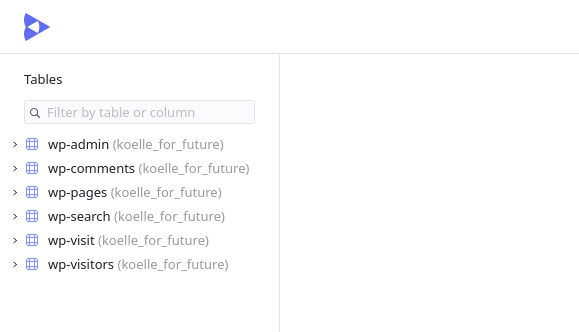
\includegraphics[width=\linewidth]{images/tables.png}
\label{fig:tablesCount}
\end{figure}
